% !TeX root = main.tex

%\setkeys{Gin}{draft}
%\onehalfspacing
	
\section{Lab Assignment Goals}

\justifying 
\par
This lab investigated the MOS differential pair composed of transistors $Q_1$ and $Q_2$ with a current mirror load formed by $Q_3$ and $Q_4$, functioning as a differential to single-ended amplifier stage. The common-mode rejection ratio (CMRR) was analyzed. The circuit was implemented using the ALD1105 MOSFET array. Differential operation was examined to evaluate its effectiveness in noise rejection and signal integrity. LTSpice simulations were performed to validate theoretical predictions and support measurement techniques.

\begin{center}
\begin{figure}[h]
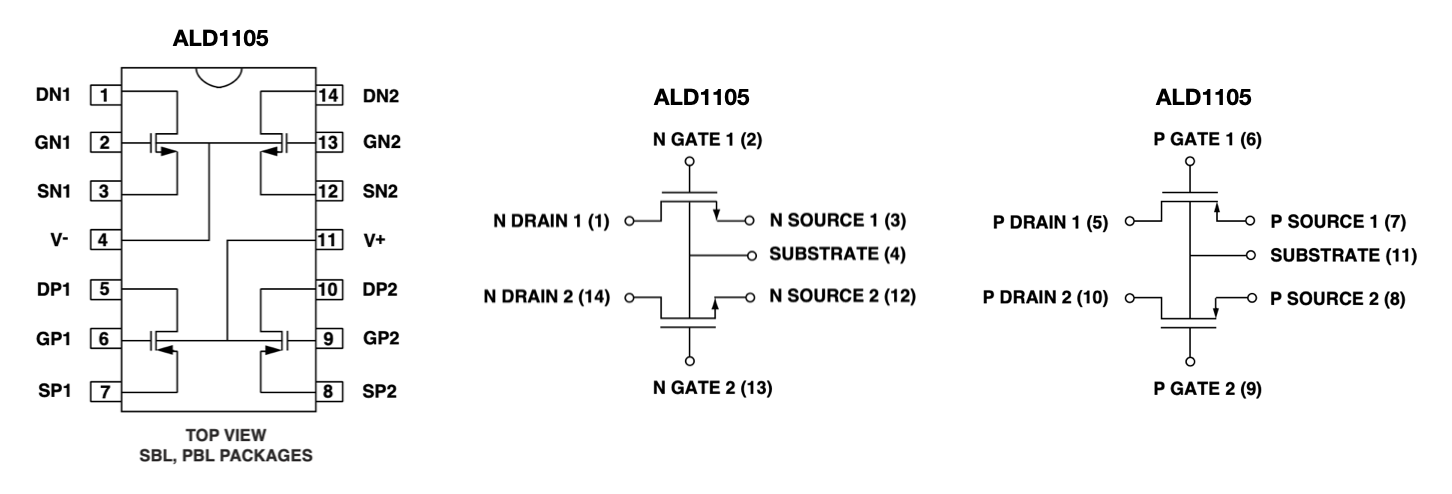
\includegraphics[scale=0.5]{Chapter_7/Lab_07_Image_1.png}
\caption{The pin-out and block diagram of the ALD1105. \textbf{Note: $V^{-}$ is the body of the NMOS devices and is connected to the source, and $V^{+}$ is the body of the PMOS devices, which is also connected to its source.}}
\label{Ch7_fig:1}
\end{figure}
\end{center}

\section{Experiment 1: MOS Differential Pair DC Measurements}

The MOS differential pair circuit was constructed on the Analog Discovery Studio as shown below:

\begin{itemize}
    \item The resistance $R_{CS}$ was measured and recorded.
    \item The DC operating point was determined by measuring node voltages and calculating the corresponding currents.
\end{itemize}

\begin{center}
\begin{circuitikz}[american,scale=0.8]
\ctikzset{tripoles/mos style=arrows}
\node at (0,9.5) {\Large \textbf{Common-Mode Input}};
\draw

(-3,0) node[nmos,scale=2] (Q1) {}
(3,0) node[nmos,scale=2,xscale=-1] (Q2) {}
(-3,5) node[pmos,scale=2, xscale=-1] (Q3) {}
(3,5) node[pmos,scale=2] (Q4) {}
(Q1.center) node[right] {$Q_{1}$}
(Q2.center) node[left] {$Q_{2}$}
(Q3.G) -- (Q4.G)
(Q1.S) -- (Q2.S)
(Q1.D) -- (Q3.D)
(Q2.D) -- (Q4.D)
(Q3.S) node[vdd] {$V_{DD}$}
(Q4.S) node[vdd] {$V_{DD}$}
(Q1.G) to[short,-o] ++(-0.5,0) node[left] {$v_{I1}$}
(Q2.G) to[short,-o] ++(0.5,0) node[right] {$v_{I2}$}
(Q1.S) to[open] ++(3,0) to[R=$R_{CS}$,*-] ++(0,-3) node[vss] {$-V_{SS}$}
(Q2.D) to[open] ++(0,0.5) to[short,*-o] ++(1,0) node[right] {$v_{O}$}
(Q1.D) to[open] ++(0,0.5) to[short,*-] ++(3,0) to[short,-*] ++(0,2.557)
;	
\end{circuitikz}

\vspace{.5cm}

$V_{DD} = 12$ V \hspace{0.5cm}  $-V_{SS} = -12$ V  \hspace{0.5cm}  $R_{CS} = 10$k $\Omega$ \hspace{0.5cm} $V_{I1}=V_{I2} = 0$ V

\vspace{.5cm}
\end{center}

\subsection*{Observations}

The simulated values for the drain currents ($I_D$) based on node voltages ($V_G$ and $V_S$) are all the same while measured values differ for the pairs formed by Q1 with Q2 and Q3 with Q4. Specifically:

\begin{itemize}
    \item \textbf{Q1/Q2 (NMOS)}: $I_D = 514.000$ $\mu\text{A}$ (simulated)
    \item \textbf{Q3/Q4 (PMOS)}: $I_D = 514.000$ $\mu\text{A}$ (simulated)
\end{itemize}

Compared to the measured values:
\begin{itemize}
    \item \textbf{Q1}: 663.487 $\mu$A,\quad \textbf{Q2}: 343.301 $\mu$A (measured)
    \item \textbf{Q3}: 663.487 $\mu$A,\quad \textbf{Q4}: 343.301 $\mu$A (measured)
\end{itemize}

\newpage

\noindent\textbf{Observations:}
\begin{itemize}
    \item The measured current for Q2 is lower than the simulated value. This discrepancy is likely due to the quadratic relationship between drain current and overdrive voltage ($V_{ov}$), which makes $I_D$ highly sensitive to small changes in $V_{ov}$, $\lambda$ is another likely candidate for as a cause behind this discrepancy \cite{rajesh_differential_2014}.
    \item Although Q2 shares the same $V_S$ and $V_{G}$ as Q1, and also taking into consideration that $I_{D3}$ and $I_{D4}$ should mirror one another, this does not result in an identical measured current. However, the measured current for Q2 is significantly lower, suggesting device mismatch or the influence of channel-length modulation (Early effect) \cite{fonstad_mit2009}.
\end{itemize}

\justifying

A MOS differential pair with a current mirror load is used to amplify differential signals while rejecting common-mode noise. This topology is foundational in analog integrated circuit design.

\begin{itemize}
    \item \textbf{Structure}: Transistors $Q_1$ and $Q_2$ form the differential pair, and $Q_3$, $Q_4$ implement the current mirror load \cite{fonstad_mit2009}.
    \[
    I_{D1} = I_{D2} = \frac{I_{R_{CS}}}{2}
    \]
    when \( V_{I1} = V_{I2} \).
    \item \textbf{Active Load Benefits}:
    \begin{itemize}
        \item Converts differential current to single-ended output \cite{rajesh_differential_2014}.
        \item Increases gain vs resistive loads:
        \[
        A_{v,d} \approx g_m \cdot R_{out} \quad \text{with } R_{out} \gg R_{resistive}
        \]
        \item Improves common-mode rejection ratio (CMRR):
        \[
        \text{CMRR} = \left| \frac{A_{d}}{A_{cm}} \right|
        \]
    \end{itemize}
    \item \textbf{Matching}:
    \begin{itemize}
        \item Requires \( Q_1 = Q_2 \) and \( Q_3 = Q_4 \) for optimal performance.
        \item Imbalances introduce input offset voltage:
        \[
        V_{OS} = \frac{I \cdot \Delta R}{2}
        \]
    \end{itemize}
    \item \textbf{Common-mode suppression}:
    \[
    V_{D1} = V_{D2} \quad \Rightarrow \quad V_O = 0 \quad \text{(ideal)}
    \]
    Common-mode gain will approach zero as the impedance of $R_{CS}$ increases \cite{deo2020bimos}.
\end{itemize}


\newpage

\section{Experiment 2: MOS Differential Pair AC Response}

The differential and common-mode gains were determined using measurement techniques, and the common-mode rejection ratio (CMRR) was calculated. The output was taken from node $v_{O}$ with respect to ground.

\begin{itemize}
    \item The differential input was applied using two synchronized sinusoidal signals, equal in magnitude but opposite in phase.
    \item The common-mode input was created by applying the same synchronized signal to both terminals with appropriate biasing.
    \item Measured resistor values were used for AC analysis in LTSpice.
    \item Measured data was recorded in the following summary tables.
\end{itemize}

% \newpage

\begin{center}
\begin{circuitikz}[american,scale=0.8]
\ctikzset{tripoles/mos style=arrows}
\node at (0,9.5) {\Large \textbf{Difference-Mode Inputs}};

\draw

(-3,0) node[nmos,scale=2] (Q1) {}
(3,0) node[nmos,scale=2,xscale=-1] (Q2) {}
(-3,5) node[pmos,scale=2, xscale=-1] (Q3) {}
(3,5) node[pmos,scale=2] (Q4) {}
(Q1.center) node[right] {$Q_{1}$}
(Q2.center) node[left] {$Q_{2}$}
(Q3.center) node[right] {$Q_{3}$}
(Q4.center) node[left] {$Q_{4}$}
(Q3.G) -- (Q4.G)
(Q1.S) -- (Q2.S)
(Q1.D) -- (Q3.D)
(Q2.D) -- (Q4.D)
(Q3.S) node[vdd] {$V_{DD}$}
(Q4.S) node[vdd] {$V_{DD}$}
(Q1.G) to[short,-o] ++(-0.5,0) node[left] {$\frac{+v_{I}}{2}$}
(Q2.G) to[short,-o] ++(0.5,0) node[right] {$\frac{-v_{I}}{2}$}
(Q1.S) to[open] ++(3,0) to[R=$R_{CS}$,*-] ++(0,-3) node[vss] {$-V_{SS}$}
(Q2.D) to[open] ++(0,0.5) to[short,*-o] ++(1,0) node[right] {$v_{O}$}
(Q1.D) to[open] ++(0,0.5) to[short,*-] ++(3,0) to[short,-*] ++(0,2.557)
;	
\end{circuitikz}

\vspace{.5cm}

$V_{DD} = 12$ V \hspace{0.5cm}  $-V_{SS} = -12$ V  \hspace{0.5cm}  $R_{CS} = 10$k $\Omega$ \hspace{0.5cm} $V_{I1}=V_{I2} = 0$ V

\vspace{.5cm}
\end{center}

\begin{itemize} 
    \item The circuit utilizes a current mirror load, which allows differential-mode current doubling and suppresses common-mode currents, making it effective for single-ended output without sacrificing gain \cite{fonstad_mit2009}.
    \item The differential-mode gain for a current mirror loaded differential pair is approximated as:
    \[
    A_{v,d} \approx \frac{2g_{m3}}{g_{o2} + g_{o4} + G_L}
    \]
\end{itemize}
\newpage
\par
where \(g_{m3}\) is the transconductance of the current mirror transistor, \(g_{o2}, g_{o4}\) are the output conductance, and \(G_L\) is the load conductance \cite{fonstad_mit2009}.
\par
\begin{itemize}
    \item In contrast, the common-mode gain is significantly smaller:
    \begin{center}
    \item $A_{v,cm} \approx \frac{g_{ob}}{2(g_{m2} + g_{o4} + G_L)}$    
    \end{center}
\end{itemize}
This results in excellent rejection of common-mode noise, contributing to a high CMRR \cite{fonstad_mit2009}.
\begin{itemize}
        
    \item From the small-signal model:
    \[
    \text{CMRR} = \frac{A_{v,d}}{A_{v,cm}} \approx \frac{2g_{m3}}{g_{ob}} \cdot \frac{g_{m2}}{g_{o2} + g_{o4} + G_L}
    \]
\end{itemize}
High values of \(g_m\) and low output conductance are favorable for achieving high CMRR \cite{fonstad_mit2009}.
\begin{itemize}
    
    \item The implementation also benefits from the mirrored topology which ensures that any common-mode signal appears equally at both inputs and is \textbf{effectively canceled out}, a principle demonstrated in both theoretical and experimental studies \cite{razaviDifferentialPair}.
    
    \item According to \cite{palermoLab6}, a finite output impedance in the tail current source slightly reduces CMRR due to common-mode to differential-mode conversion:
    \[
    A_{cm} \approx \frac{1}{1 + 2g_mR_{SS}}
    \]
    \item (for this experiment, $R_{SS} = R_{CS}$)
\end{itemize}
where \(R_{SS}\) is the source degeneration resistance. Ideally, this should be large.
\begin{itemize}
    \item The presence of mismatches (e.g., \(g_{m1} \neq g_{m2}\)) introduces additional differential components into the output in response to a purely common-mode input, reducing CMRR. This is quantified using:
    \[
    A_{CM \to DM} \approx \frac{(g_{m1} - g_{m2}) R_{SS}}{g_{m1} + g_{m2} + \dots}
    \]
    which highlights the importance of symmetric layout and transistor matching 
\cite{iiitd_lecture16}.
\end{itemize}

\begin{itemize}
    \item Overall, using a current mirror as an active load provides significant advantages in terms of:
        \begin{itemize}
            \item Converting differential signal to single-ended output efficiently
            \item Doubling the effective gain compared to resistive loads
            \item Minimizing common-mode gain
            \item Enabling high CMRR with compact layout
        \end{itemize}
    as emphasized in multiple foundational sources \cite{rajesh_differential_2014, fonstad_mit2009, iiitd_lecture16}.
\end{itemize}


\newpage

\begin{center}

\begin{table}[H]
\begin{tabular}{ | >{\centering\arraybackslash} m{2.5cm} | >{\centering\arraybackslash} m{2.5cm} |  >{\centering\arraybackslash} m{2.5cm} | >{\centering\arraybackslash} m{2.5cm} | >{\centering\arraybackslash} m{2.5cm} |}
\hline
\multicolumn{5}{|c|}{DC Operating Point}        \\ \hline
Device & Quantity & Simulated  & Measured & Units \\ \hline
\multirow{5}{*}{$Q_{1}$} & $I_{D}$ & 514.000 & 540.335 & $\mu$A   \\ \cline{2-5} 
& $|V_{OV}|$ & 1.267 & 1.365 & V \\ \cline{2-5} 
& $V_{G}$ & 0.000 & 0.000 & V  \\ \cline{2-5} 
& $V_{D}$ & 9.010 & 8.606 & V \\ \cline{2-5} 
& $V_{S}$ & -1.844 & -1.985 & V \\ \hline

\multirow{5}{*}{$Q_{2}$} & $I_{D}$  & 514.000 & 540.335 & $\mu$A   \\ \cline{2-5} 
& $|V_{OV}|$ & 1.267 & 1.365 & V \\ \cline{2-5} 
& $V_{G}$ & 0.000 & 0.000 & V  \\ \cline{2-5} 
& $V_{D}$ & 9.011 & 8.606 & V \\ \cline{2-5} 
& $V_{S}$ & -1.844 & -1.985 & V \\ \hline

\multirow{5}{*}{$Q_{3}$} & $I_{D}$  & 514.000 & 540.335 & $\mu$A   \\ \cline{2-5} 
& $|V_{OV}|$ & 2.343 & 2.394 & V \\ \cline{2-5} 
& $V_{G}$ & 9.010 & 8.606 & V  \\ \cline{2-5} 
& $V_{D}$ & 9.010 & 8.606 & V \\ \cline{2-5} 
& $V_{S}$ & 12.000 & 12.000 & V \\ \hline

\multirow{5}{*}{$Q_{4}$} & $I_{D}$  & 514.000 & 540.335 & $\mu$A   \\ \cline{2-5} 
& $|V_{OV}|$ & 2.343 & 2.394 & V \\ \cline{2-5} 
& $V_{G}$ & 9.010 & 8.606 & V  \\ \cline{2-5} 
& $V_{D}$ & 9.010 & 8.606 & V \\ \cline{2-5} 
& $V_{S}$ & 12.000 & 12.000 & V \\ \hline
\end{tabular}
\caption{DC Summary Table}
\end{table}

\newpage

\begin{table}[H]
\begin{tabular}{ | >{\centering\arraybackslash} m{2.5cm} | >{\centering\arraybackslash} m{2.5cm} |  >{\centering\arraybackslash} m{2.5cm} |}
\hline
Quantity & Measured & Units \\ \hline
$R_{CS}$ & 9.872 & k$\Omega$ \\ \hline
\end{tabular}
\caption{Resistor Summary}	
\end{table}

\begin{table}[H]
\begin{tabular}{ | >{\centering\arraybackslash} m{3.5cm} |  >{\centering\arraybackslash} m{3cm} | >{\centering\arraybackslash} m{3cm} | >{\centering\arraybackslash} m{2cm} |}
\hline
\multicolumn{4}{|c|}{AC Summary - Single Ended}        \\ \hline
Quantity & Simulated  & Measured & Units \\ \hline
$A_{d}$  & 44.888 & 24.161 & V/V   \\ \cline{1-4} 
$A_{d}$ & 33.040 & 27.662 & dB \\ \hline
$A_{cm}$  & 0.105 & 0.183 & V/V   \\ \cline{1-4}
$A_{cm}$ & -19.591 & -14.751 & dB \\ \hline
CMRR  & 52.632 & 42.413 & dB   \\ \cline{1-4}
\end{tabular}
\caption{AC Summary Table - Single Ended Output}
\end{table}
\end{center}
\newpage

\begin{figure}
    \centering
    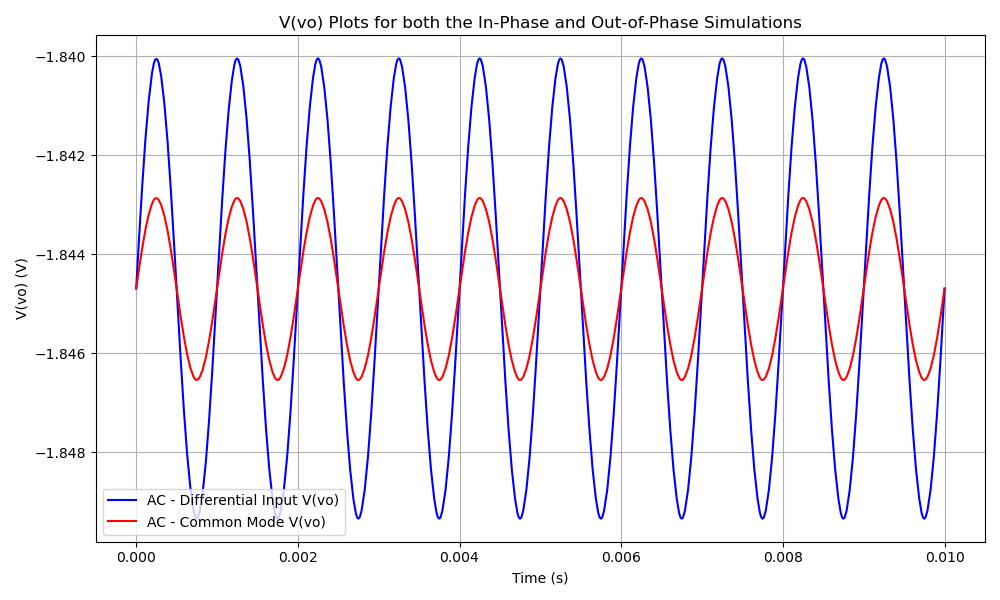
\includegraphics[width=0.95\linewidth]{Chapter_7/Lab_07_CM_vs_Diff_Plot.png}
    \caption{Differential Mode V(vo)}
    \label{Ch7_fig:2}
\end{figure}
\clearpage

\begin{figure}
    \centering
    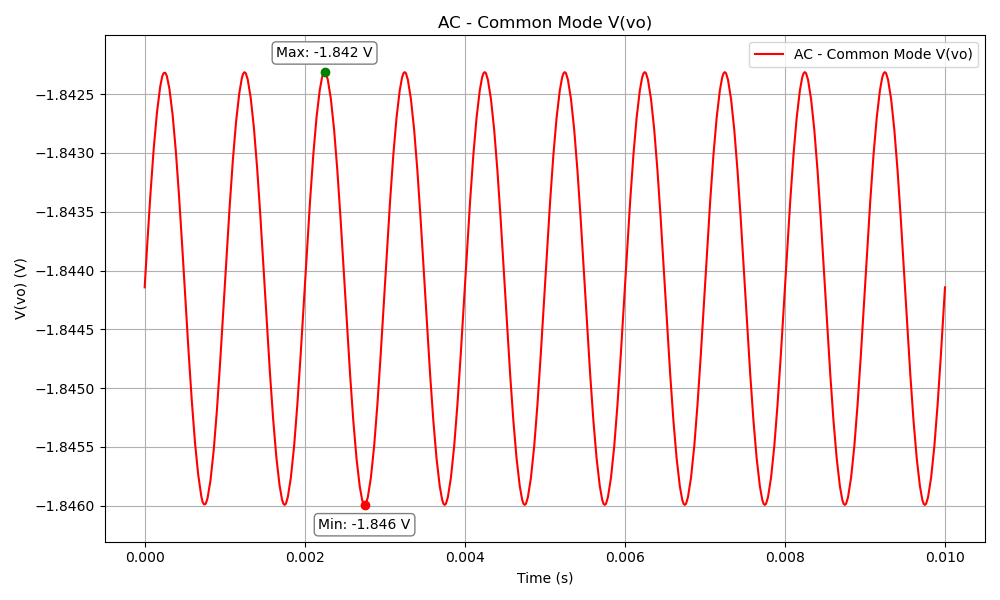
\includegraphics[width=0.95\linewidth]{Chapter_7/Lab_07_AC_CommonMode_vo_Plot.png}
    \caption{Common Mode V(vo)}
    \label{Ch7_fig:3}
\end{figure}
\clearpage

%\newpage
%\section*{Python Code used in Calculations}
%\lstinputlisting[language=Python]{Appendix/Python_Code/Lab_07_Table_1_DC_Summary_Placzek.py}
%\clearpage
\section{Python	Output: Simulated vs Measured \% Difference}
\vspace{0.25cm}
\begin{verbatim}
	|--------------------------------------------------------|
	|============== DC Percent Difference Table =============|
	| Dev | Quant |  Sim   | Meas  | Unit | Diff  | %Diff    |
	|-----|-------|--------|-------|------|-------|----------|
	| Q1  | ID    | 514.0  | 540.3 | uA   | 26.3  | 5.116    |
	| Q1  | VOV   | 1.267  | 1.365 | V    | 0.098 | 7.733    |
	| Q1  | VG    | 1.840  | 0.000 | V    | 1.840 | N/A  |
	| Q1  | VD    |10.900  | 8.606 | V    | 2.294 | 21.038   |
	| Q1  | VS    | 0.000  |-1.985 | V    | 1.985 | N/A      |
	| Q2  | ID    | 514.0  | 540.3 | uA   | 26.3  | 5.116    |
	| Q2  | VOV   | 1.267  | 1.365 | V    | 0.098 | 7.733    |
	| Q2  | VG    | 1.840  | 0.000 | V    | 1.840 | 100.000  |
	| Q2  | VD    |10.900  | 8.606 | V    | 2.294 | 21.038   |
	| Q2  | VS    | 0.000  |-1.985 | V    | 1.985 | N/A      |
	| Q3  | ID    | 514.0  | 540.3 | uA   | 26.3  | 5.116    |
	| Q3  | VOV   | 2.343  | 2.394 | V    | 0.051 | 2.177    |
	| Q3  | VG    |-2.990  | 8.606 | V    |11.596 | 388.125  |
	| Q3  | VD    |-2.990  | 8.606 | V    |11.596 | 388.125  |
	| Q3  | VS    | 0.000  |12.000 | V    |12.000 | N/A      |
	| Q4  | ID    | 514.0  | 540.3 | uA   | 26.3  | 5.116    |
	| Q4  | VOV   | 2.343  | 2.394 | V    | 0.051 | 2.177    |
	| Q4  | VG    |-2.990  | 8.606 | V    |11.596 | 388.125  |
	| Q4  | VD    |-2.990  | 8.606 | V    |11.596 | 388.125  |
	| Q4  | VS    | 0.000  |12.000 | V    |12.000 | N/A      |
	|--------------------------------------------------------|
	|========================================================|
\end{verbatim}

\section{Python Code Listings}

The Python implementations for the current mirror analysis can be found in the Appendix: DC Summary Calculations (\cref{lst:Ch7:List1}), AC Summary Calculations (\cref{lst:Ch7:List2}), and Data Analysis and Plots (\cref{lst:Ch7:List3}).

\section{Conclusion}
\vspace{0.25cm}
\justifying
This lab demonstrated the operation and advantages of a MOSFET differential pair using the ALD1105 IC. By constructing and analyzing the circuit both experimentally and through LTSpice simulations, we verified that differential signaling offers significant benefits over single-ended approaches. Notably, the differential configuration achieved a much higher common-mode rejection ratio (CMRR), with simulated and measured values of approximately $59.9$ dB and $48.3$ dB respectively, compared to $17.1$ dB and $21.7$ dB for single-ended output. These results confirm the superior noise rejection capabilities inherent to differential systems. Theoretical modeling was reinforced by close agreement between simulated and measured values for parameters such as differential gain and DC operating points. Overall, this lab emphasized the importance of differential signaling in high-fidelity analog design and the utility of simulation tools in predicting and optimizing circuit performance.

\clearpage
\printbibliography[heading=subbibliography]